\chapter{Redes neuronales y YOLO sin complicaciones}

\begin{enpocas}
Qué es aprender a partir de ejemplos, cómo funciona una neurona artificial, qué hace una convolución,
cómo detecta objetos YOLO, cómo se entrena (datos, etiquetas, épocas, pérdida) y cómo se mide qué tan
bien funciona (IoU, precisión, recall, mAP).
\end{enpocas}

\section{Programar contra aprender}

¿Cómo le explicarías a una computadora qué es el humo? Podrías intentar reglas: ``muchos píxeles
grises claros juntos''. Pero las nubes también lo son, y el humo a contraluz es oscuro. Las reglas
escritas a mano fallan pronto. El \textbf{aprendizaje automático} hace lo contrario: se le dan miles de
ejemplos con la respuesta correcta (``aquí hay humo, en este rectángulo'') y el programa ajusta sus
propios parámetros hasta acertar. Eso es \textbf{entrenar}.

\section{La neurona artificial}

\begin{figure}[H]
\centering
\begin{tikzpicture}[
  n/.style={circle,draw,fill=#1,minimum size=0.8cm,inner sep=0},n/.default=blue!12,
  fl/.style={-{Stealth[length=2mm]}}]
  \foreach \i/\t in {1/$x_1$,2/$x_2$,3/$x_3$} { \node (x\i) at (0,-\i*1.1) {\t}; }
  \node[n=orange!20,minimum size=1.3cm] (s) at (3,-2.2) {$\sum$};
  \node[draw,rounded corners,fill=green!12] (f) at (5.2,-2.2) {activación};
  \node (y) at (7.3,-2.2) {salida};
  \foreach \i/\w in {1/$w_1$,2/$w_2$,3/$w_3$} { \draw[fl] (x\i) -- node[above,font=\scriptsize]{\w} (s); }
  \node (b) at (3,-0.4) {$b$ (sesgo)}; \draw[fl] (b) -- (s);
  \draw[fl] (s) -- (f); \draw[fl] (f) -- (y);
  % red
  \begin{scope}[xshift=9.5cm,yshift=-0.4cm]
    \foreach \i in {1,...,4} \node[n] (a\i) at (0,-\i*0.9) {};
    \foreach \i in {1,...,5} \node[n=orange!20] (b\i) at (1.8,-\i*0.9+0.45) {};
    \foreach \i in {1,...,3} \node[n=green!15] (c\i) at (3.6,-\i*0.9-0.45) {};
    \foreach \i in {1,...,4} \foreach \j in {1,...,5} \draw[black!35] (a\i) -- (b\j);
    \foreach \i in {1,...,5} \foreach \j in {1,...,3} \draw[black!35] (b\i) -- (c\j);
    \node[font=\scriptsize] at (0,-4.4) {entrada}; \node[font=\scriptsize] at (1.8,-4.4) {capa oculta}; \node[font=\scriptsize] at (3.6,-4.4) {salida};
  \end{scope}
\end{tikzpicture}
\caption{Izquierda: una neurona multiplica cada entrada por un \emph{peso}, suma todo y pasa el
resultado por una función de activación. Derecha: una red son muchas neuronas en capas.}
\end{figure}

Una neurona artificial hace una cuenta muy simple:
\begin{equation}
\text{salida} = \text{activación}\big(w_1x_1 + w_2x_2 + \dots + w_nx_n + b\big).
\end{equation}
Los \textbf{pesos} $w_i$ dicen qué tan importante es cada entrada. Sola, una neurona es poca cosa;
millones de ellas en capas pueden reconocer caras, voces o fuego. Entrenar es buscar los pesos que
hacen que la red acierte. YOLO26n tiene unos 2.5 millones de pesos.

\section{Convoluciones: buscar patrones locales}

Conectar cada píxel con cada neurona sería enorme. Las redes para imágenes usan
\textbf{convoluciones}: un filtro pequeño (por ejemplo $3\times3$ números) que se desliza por toda la
imagen; en cada posición multiplica sus números por los píxeles de abajo y suma. Según los números del
filtro, resalta bordes, manchas, texturas...

\begin{figure}[H]
\centering
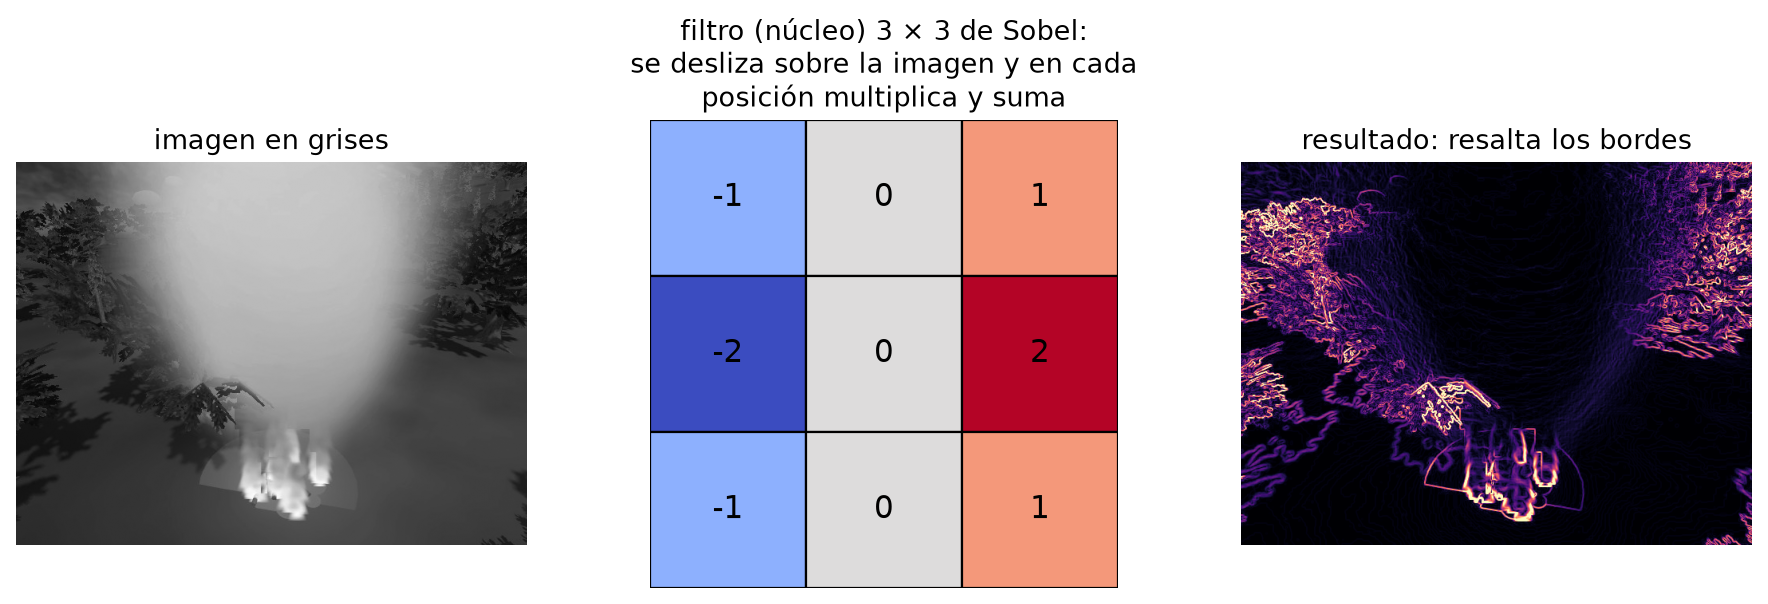
\includegraphics[width=\textwidth]{c_convolucion.png}
\caption{Un filtro de bordes (Sobel) aplicado a la imagen del incendio. En una red convolucional los
números de los filtros no se eligen a mano: se aprenden.}
\end{figure}

Una \textbf{red convolucional} (CNN) apila muchas capas de filtros: las primeras detectan bordes y
colores, las intermedias texturas (llamas, humo, hojas) y las últimas objetos completos.

\section{Detectar objetos: cajas y clases}

Hay varias tareas de visión: \emph{clasificar} (¿hay fuego en la imagen?), \emph{detectar} (¿dónde?)
y \emph{segmentar} (¿qué píxeles exactamente?). Necesitamos \textbf{detección}: el dron debe saber en
qué parte de la imagen está el fuego para calcular hacia dónde está. Un detector entrega una lista de
\textbf{cajas} (rectángulos), cada una con una \textbf{clase} (``fuego'' o ``humo'') y una
\textbf{confianza} entre 0 y 1.

\section{YOLO}

\textbf{YOLO} (\emph{You Only Look Once}, ``solo miras una vez'') es una familia de detectores muy
rápida: en lugar de revisar la imagen por pedazos, una sola pasada de la red predice todas las cajas a
la vez. Por eso sirve en tiempo real, incluso en un dron. Usamos \textbf{YOLO26n}, la versión más
reciente de Ultralytics en su tamaño más pequeño (\emph{nano}); en la GPU procesa una imagen en pocos
milisegundos.

\begin{figure}[H]
\centering
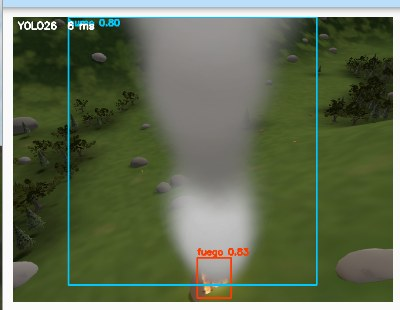
\includegraphics[width=0.55\textwidth]{yolo_panel.jpg}
\caption{Lo que entrega YOLO: cajas con su clase y su confianza (``fuego 0.83'').}
\end{figure}

\section{Entrenar: datos, etiquetas y épocas}

\begin{description}
  \item[Dataset:] el conjunto de imágenes de ejemplo. Se usaron 6000 imágenes del simulador.
  \item[Etiquetas:] para cada imagen, las cajas correctas. En formato YOLO, un archivo de texto con
        una línea por objeto: clase y caja (centro, ancho y alto, como fracción de la imagen).
  \item[Entrenamiento y validación:] el dataset se parte en dos. La red aprende con uno
        (\emph{entrenamiento}) y se evalúa con el otro, que nunca ve al aprender (\emph{validación}).
        Así se mide si generaliza o solo memoriza.
  \item[Época:] una pasada completa por todas las imágenes de entrenamiento. Se hicieron 60.
  \item[Pérdida (loss):] un número que mide qué tan mal predice la red. Entrenar es bajarla, ajustando
        los pesos un poquito en la dirección que la reduce (\emph{descenso de gradiente}).
  \item[Ajuste fino (fine-tuning):] no se empezó de cero, sino de una red ya entrenada con el dataset
        COCO (80 clases de objetos comunes). La red ya sabe ``ver'' y solo aprende las clases nuevas.
\end{description}

\begin{figure}[H]
\centering
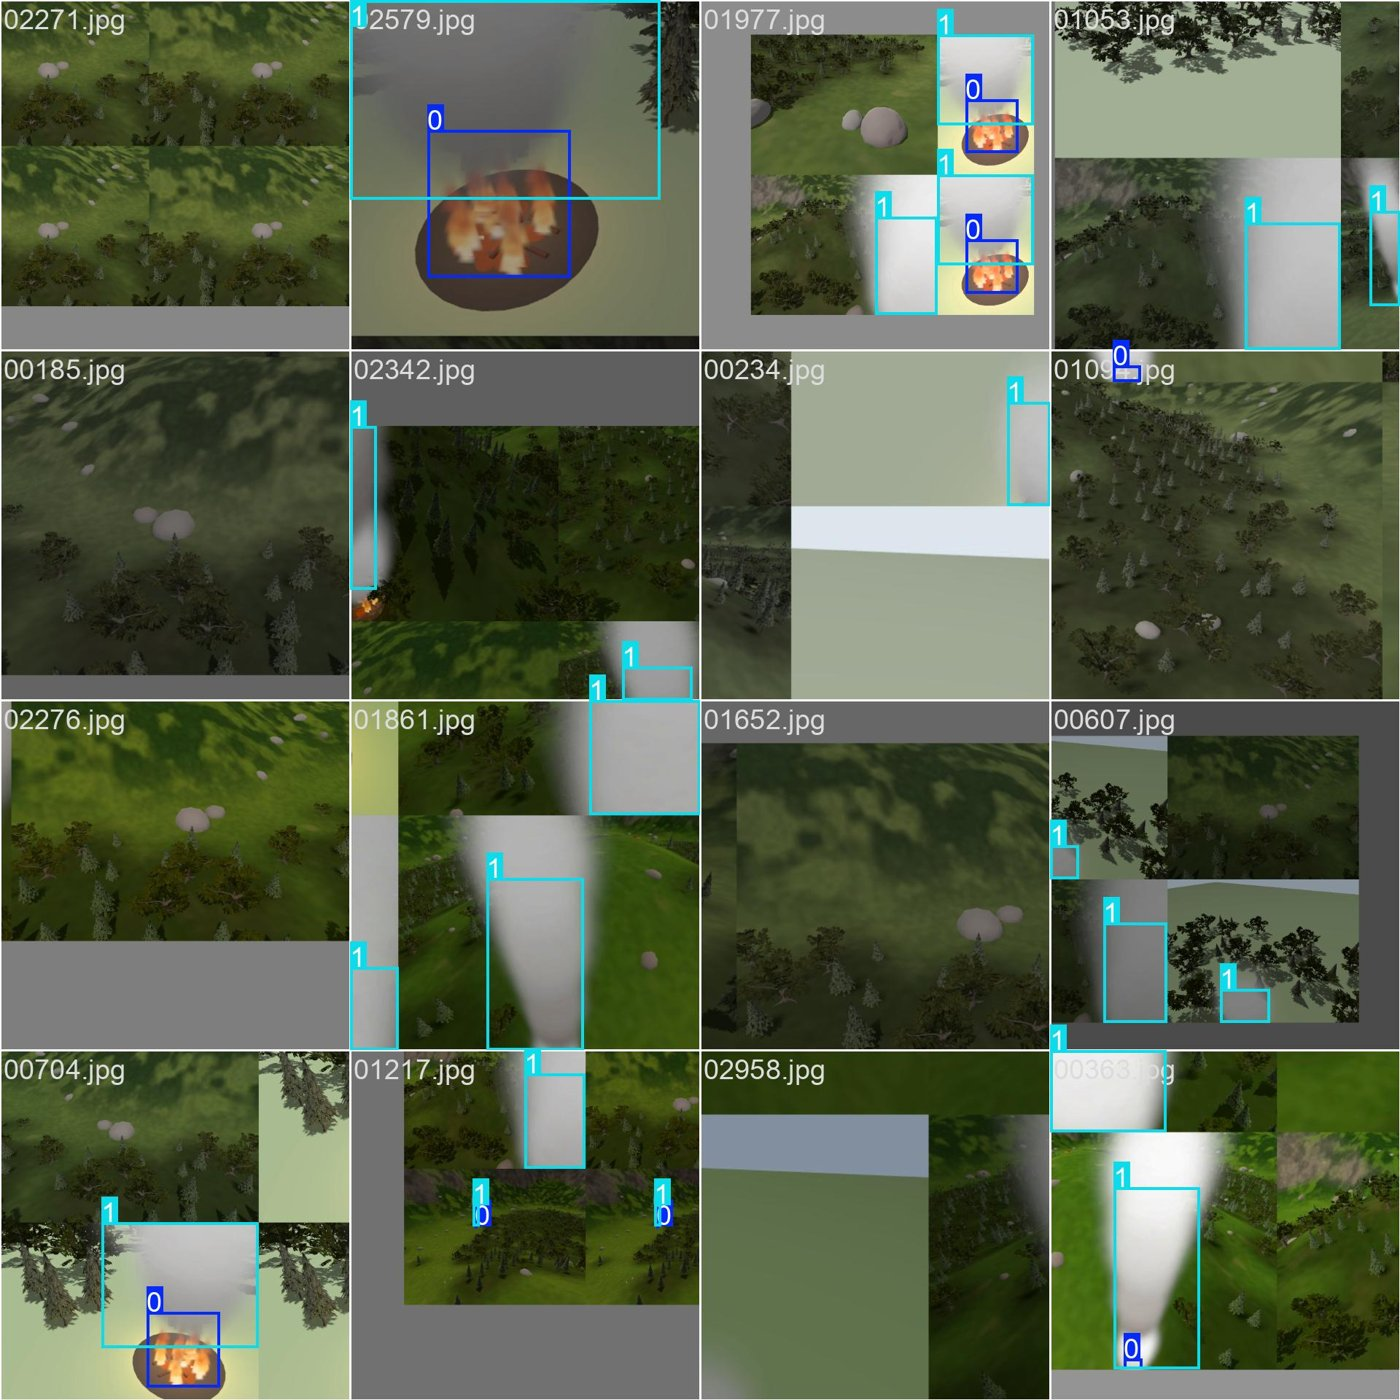
\includegraphics[width=0.85\textwidth]{yolo_lote_etiquetas.jpg}
\caption{Un lote de imágenes de entrenamiento con sus etiquetas. Las imágenes se alteran al azar
(mosaicos, cambios de color y escala) para que la red no memorice.}
\end{figure}

\begin{tecnico}
Etiquetar 6000 imágenes a mano tomaría días. Como en el simulador sabemos dónde está el fuego, las
etiquetas se calcularon solas: se proyecta con el modelo estenopeico una nube de puntos del volumen de
las llamas y del humo, se descartan los puntos tapados por árboles o por el terreno, y la caja es el
rectángulo que encierra los puntos visibles (capítulo~\ref{cap:yolo-sim}).
\end{tecnico}

\section{Cómo se mide si funciona}

\subsection{IoU: ¿le atinó a la caja?}

Una predicción cuenta como acierto si su caja se parece lo bastante a la verdadera. Se mide con la
\textbf{intersección sobre unión} (IoU):

\begin{figure}[H]
\centering
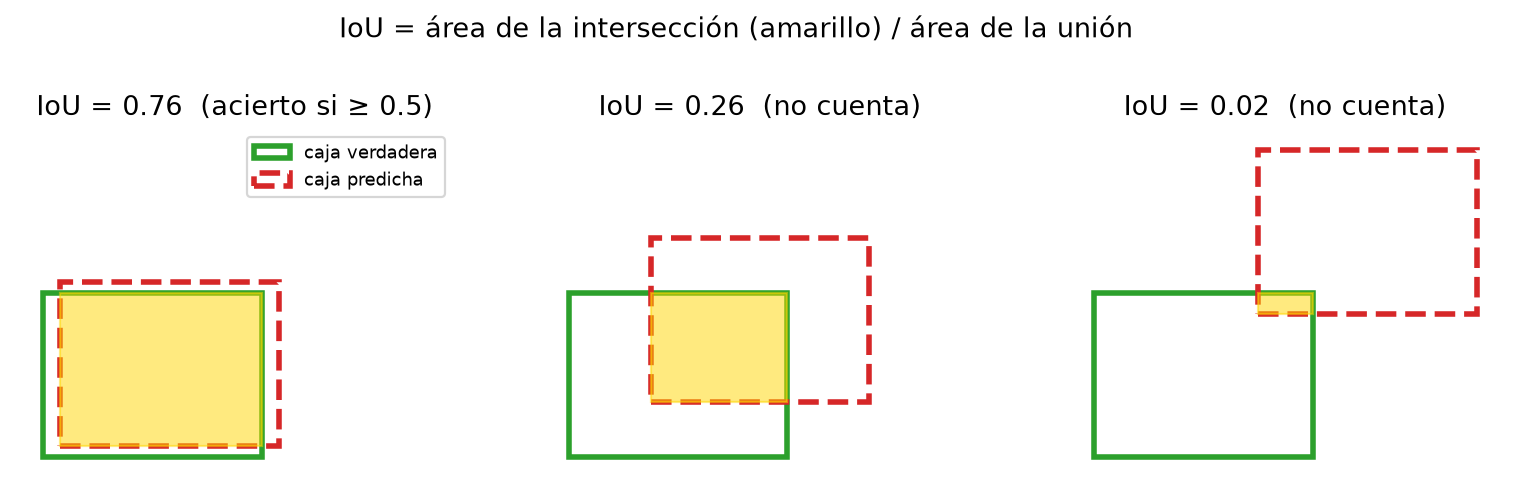
\includegraphics[width=\textwidth]{c_iou.png}
\caption{IoU: 1 es perfecta, 0 es no tocarse. Normalmente se exige al menos 0.5.}
\end{figure}

\subsection{Precisión y recall}

\begin{description}
  \item[Verdadero positivo (VP):] dijo ``fuego'' y había fuego.
  \item[Falso positivo (FP):] dijo ``fuego'' y no había (por ejemplo, una roca oscura).
  \item[Falso negativo (FN):] había fuego y no lo vio.
\end{description}
\begin{align}
\text{precisión} &= \frac{VP}{VP + FP} && \text{(cuando dice ``fuego'', ¿cuántas veces acierta?)}\\
\text{recall} &= \frac{VP}{VP + FN} && \text{(de los fuegos que hay, ¿cuántos encuentra?)}
\end{align}

\begin{ejemplo}
Una alarma de humo muy sensible tiene buen recall (no se le escapa ningún incendio) pero mala precisión
(suena cuando quemas pan tostado). Una muy poco sensible, al revés. Para un dron que vigila un bosque
importan las dos: no queremos ignorar un incendio, pero tampoco mandar a los bomberos a ver una roca.
\end{ejemplo}

\subsection{mAP}

La \textbf{precisión media} (AP) resume la curva de precisión contra recall al variar el umbral de
confianza; promediada entre clases es la \textbf{mAP}. \emph{mAP50} usa IoU $\ge$ 0.5; \emph{mAP50-95}
promedia exigencias de IoU de 0.5 a 0.95 (cajas más ajustadas). Nuestro modelo final: mAP50 = 0.988 y
mAP50-95 = 0.881, precisión 0.97 y recall 0.95.

\begin{figure}[H]
\centering
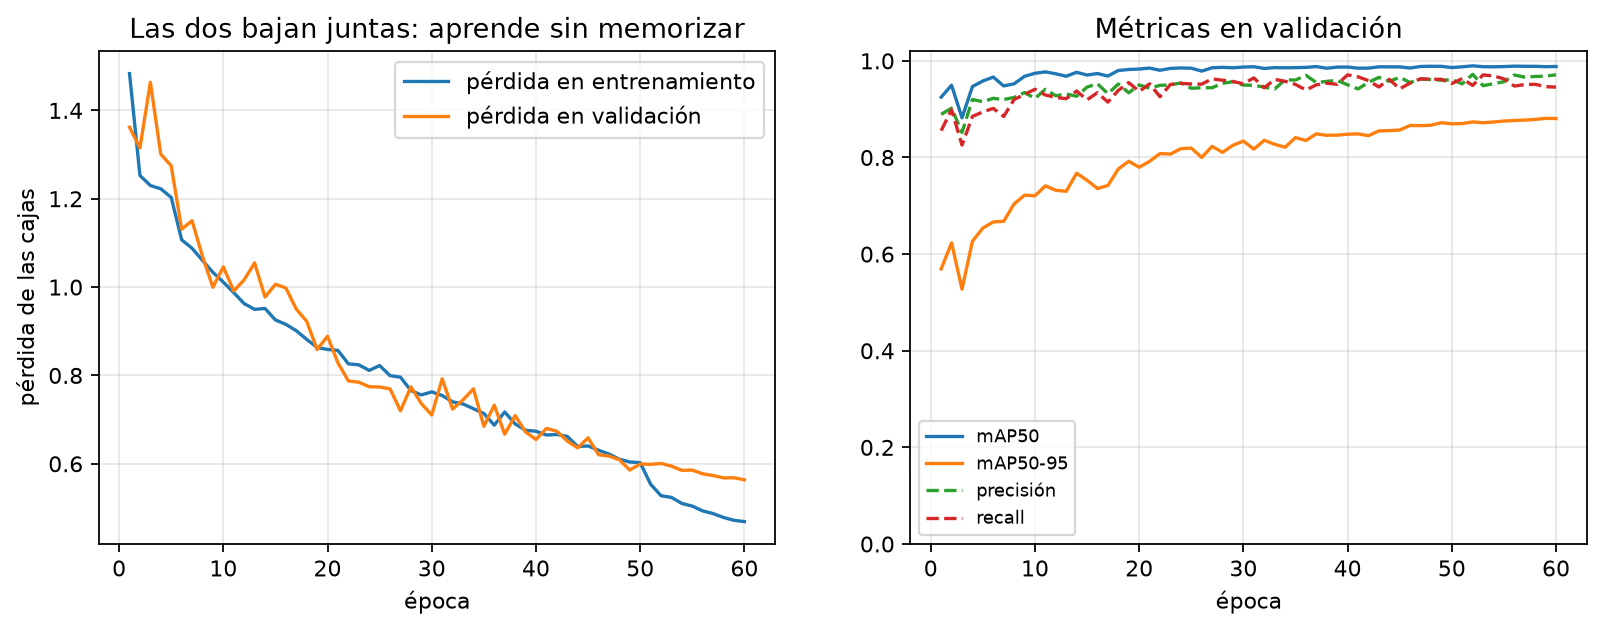
\includegraphics[width=\textwidth]{c_entrenamiento.png}
\caption{Izquierda: la pérdida baja en entrenamiento y en validación a la par (no hay
sobreajuste). Derecha: las métricas suben y se estabilizan.}
\end{figure}

\section{Sobreajuste y por qué importan los datos}

Si la red memoriza las imágenes de entrenamiento en lugar de aprender el concepto, le va muy bien con
ellas y mal con imágenes nuevas: eso es \textbf{sobreajuste}. Se detecta porque la pérdida de
validación deja de bajar o sube. Más importante aún: \textbf{la red solo sabe lo que vio}.

\begin{leccion}
El primer modelo se entrenó solo con el mundo \cod{bosque} (plano, sin rocas grandes). En el mundo
grande confundió una roca oscura con fuego: nunca había visto una roca. Se agregaron 3000 imágenes del
mundo grande, una de cada cinco apuntando a rocas o animales sin fuego, y el problema desapareció.
\end{leccion}

\begin{aviso}
Un modelo entrenado solo con imágenes de simulación probablemente fallará con fuego real: los colores,
la luz y el humo reales son distintos. Antes de volar el dron de verdad hay que reentrenar con imágenes
reales (por ejemplo, el dataset D-Fire).
\end{aviso}
